% !TeX root = ../thuthesis-example.tex

\chapter{实验与算法应用}

在这个章节中,我们将我们的验证与综合方法应用至受控Van der Pol振荡器上。我们首先考虑了没有加性不确定性的受控Van der Pol振荡器(章节~\ref{sec:cleanvanderpol}),并且表明我们的算法能够复现~\cite{clark22arxiv-cbf}中的圆形控制障碍函数(章节~\ref{sec:uncertainvanderpol})。而当不确定性存在时,我们展示了如何综合出一系列椭圆形的鲁棒控制障碍函数,它们能够产生一系列严格为正的值函数。

\section{无加性不确定性的受控Van der Pol振荡器}
\label{sec:cleanvanderpol}

考虑一个无加性不确定性的Van der Pol振荡器~\cite{clark22arxiv-cbf}
\begin{equation}\label{eq:cleanvdpodynamics}
    \dot{x} = \left[ \begin{array}{c}
        \dot{x}_1 \\ \dot{x}_2
    \end{array} \right] 
    = \left[ \begin{array}{c}
        x_2 \\
        \frac{1}{2}(1 - x_2^2) x_2 - x_1
    \end{array} \right]
    + \left[ \begin{array}{c}
        0 \\ x_1
    \end{array} \right] u
\end{equation}
令
\begin{equation}\label{eq:cleanvdpou}
    \mathbb{U} = \left\{ u \in \mathbb{R} \mid u^2 - u_{\max}^2 \le 0 \right\}
\end{equation}

定义以下候选的圆形控制障碍函数
\begin{equation}
    \label{eq:cleanvdpocbf}
    b(x, \theta) = \theta - \parallel x \parallel^2, \quad \theta \in \Theta := [0, \theta_{\max}]
\end{equation}
很明显,假设~\ref{assume:archimedeanness}成立。在附录~\ref{app:bound:y:cleanvdp}中,我们计算了多项式优化问题中~\eqref{eq:verifypop}中$y$的界。

\subsection{验证问题}
我们选取了$u_{\max} = 5$,$\theta_{\max} = 2$,并且选取了$\kappa = 4$作为验证多项式优化问题~\eqref{eq:verifypop}中半正定松弛的度。
\footnote{
    我们采用了\url{https://github.com/MIT-SPARK/CertifiablyRobustPerception}中提供的半正定优化松弛算法,并且使用了MOSEK这一求解器。
}
图像~\ref{fig:vanderpol_clean}(a)中,蓝色的点状线条刻画了$\theta = 0, 0.1, 0.2, \dots, 2.0$这些采样点处,半正定松弛所得到的解。在所有这些情况下,半正定松弛是紧的,并且它们能还原出验证多项式优化问题~\eqref{eq:standardpop}的最优解。例如,当$\theta = 0.1$时,$x^\star = [0; \pm 0.3162]$能够取得全局最小值$V(\theta) = -0.09$;当$\theta = 1.1$时,$x^\star = [\pm 1.0488; 0]$能够取得全局最小值$V(\theta) = 0$。从图像~\ref{fig:vanderpol_clean}(a)中的蓝色点状线条,我们还可以观察到$b(x, \theta)$是一个合法的控制障碍函数,当且仅当$\theta = 0$或者$\theta \ge 1$,这些结论与~\cite{clark22arxiv-cbf}相符。然而,我们的算法能够在其它方面比~\cite{clark22arxiv-cbf}中的算法做得更好:当$b(x, \theta)$不是合法的控制障碍函数时(亦即,$\theta \in (0, 1)$),我们的算法能够还原出使得$V(\theta)$为负数的$x^\star$,然而基于平方和的优化方法~\cite{clark22arxiv-cbf}在这种情况下不可行(亦即,不可解),且无法返回一个“见证值”$x^\star$。

%!TEX root = ../thuthesis-example.tex

\begin{figure}
    \centering
    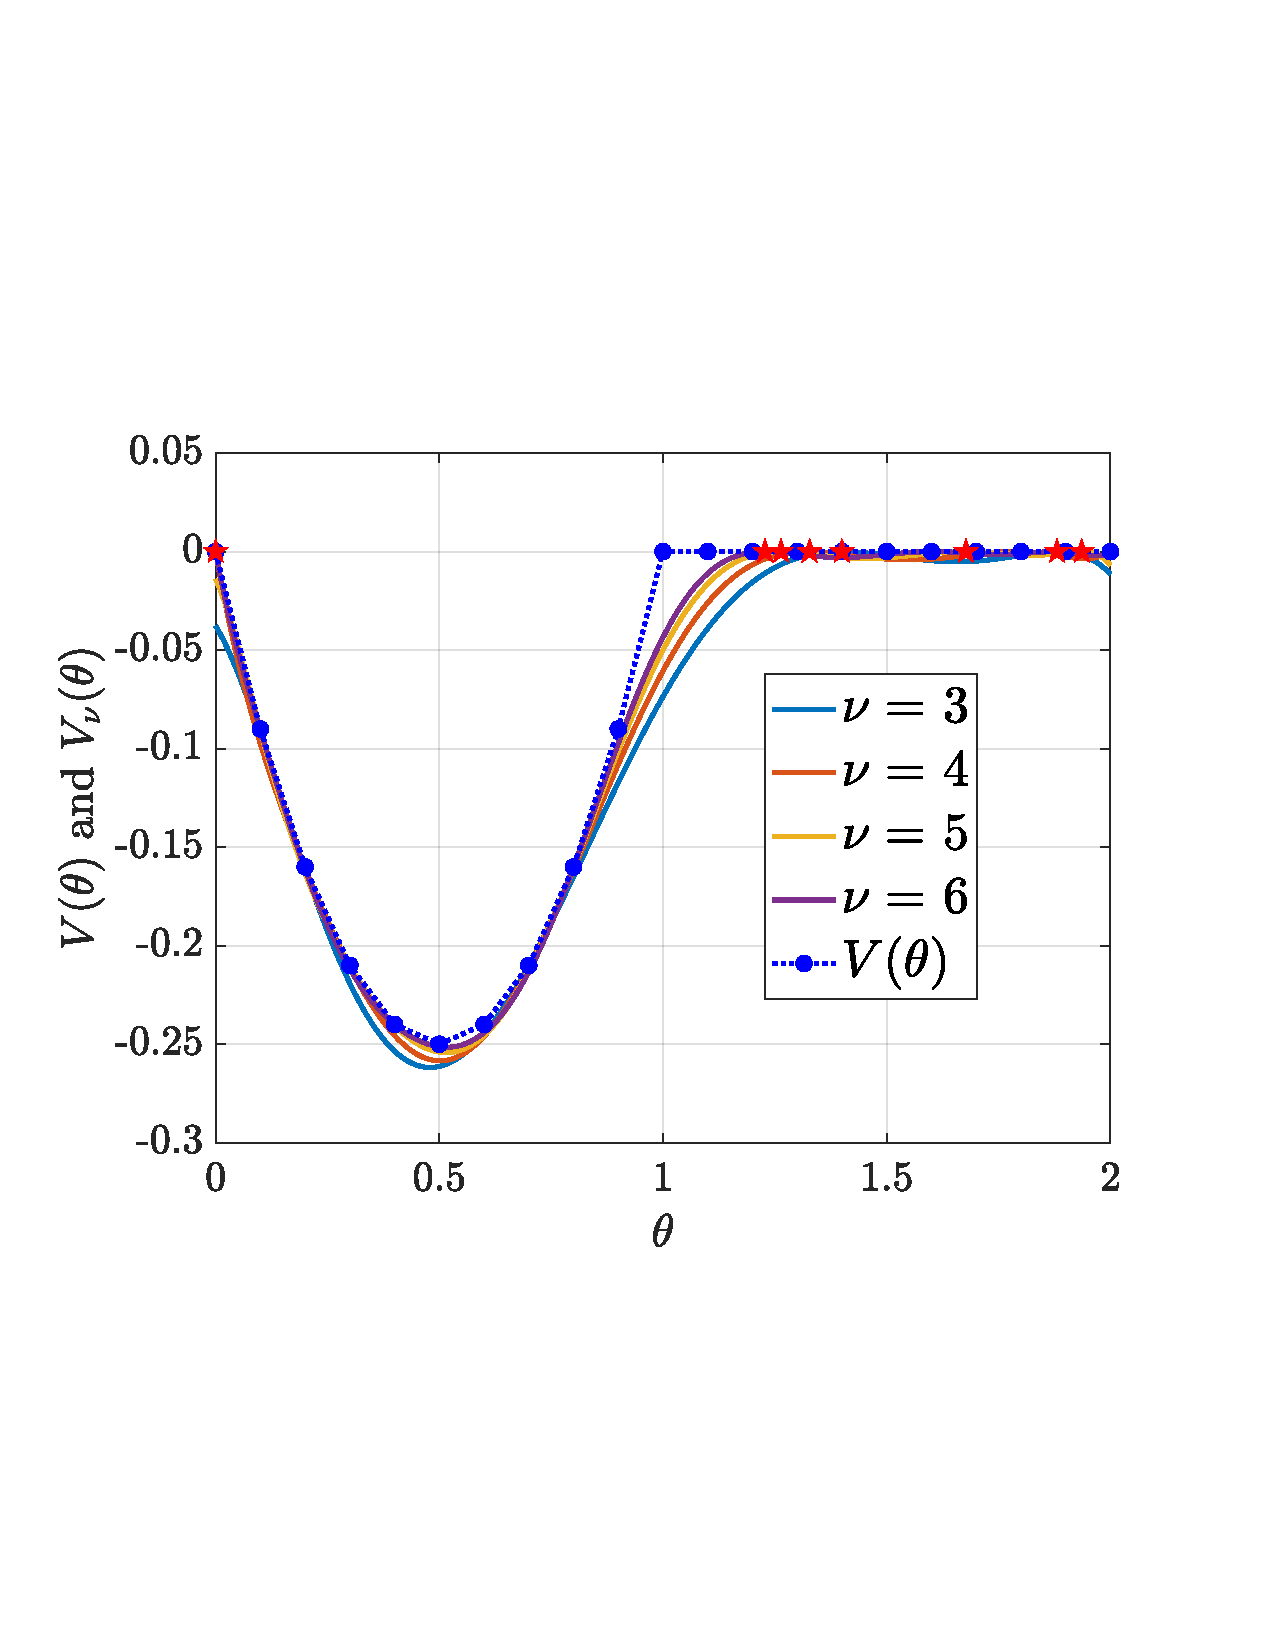
\includegraphics[width=0.65\columnwidth]{vanderpol_clean.pdf} \\
    (a) $\Theta = [0,2]$ \\

    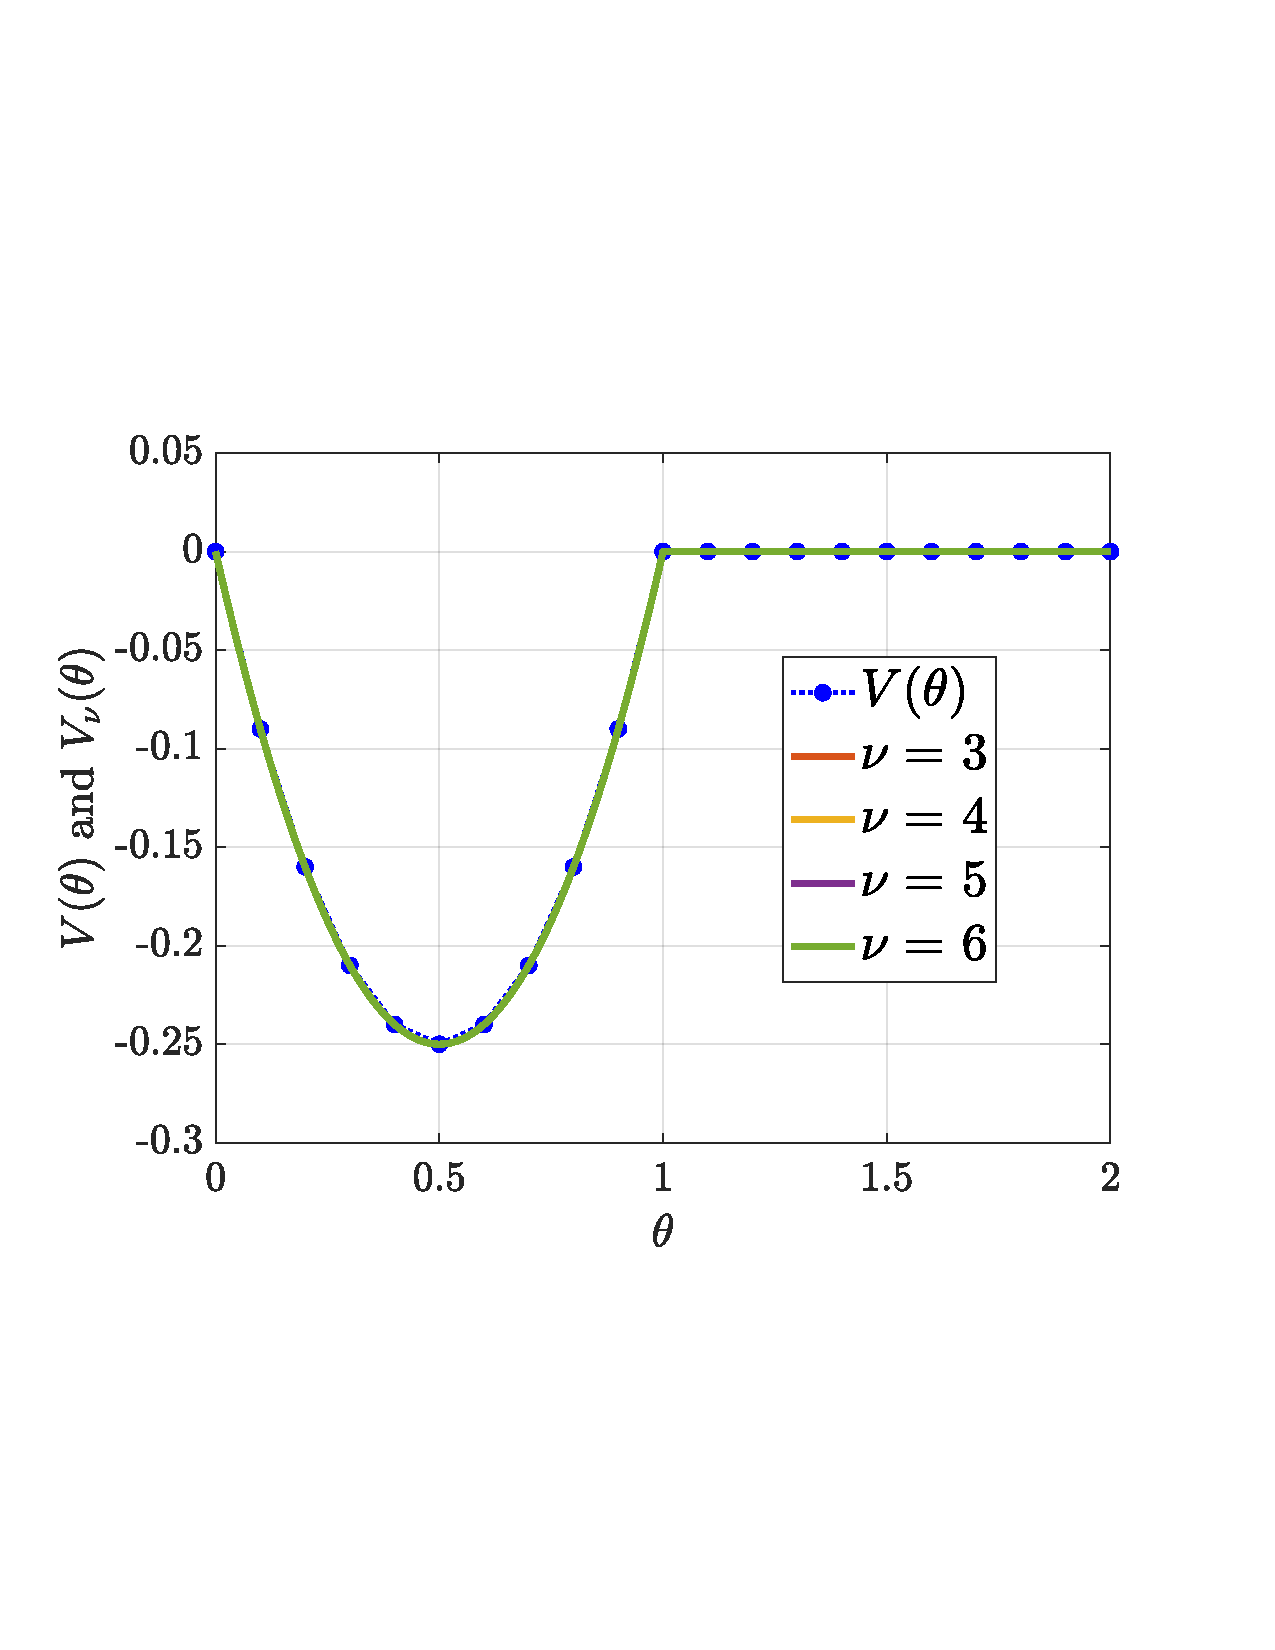
\includegraphics[width=0.65\columnwidth]{vanderpol_clean_refine.pdf} \\
    (b) $\Theta_1 = [0,1]$与$\Theta_2 = [1,2]$

    \caption{
        无不确定性的受控Van der Pol振荡器中,圆形控制障碍函数$b(x,\theta) = \theta - \parallel x \parallel^2$的验证与综合问题~\eqref{eq:cleanvdpodynamics}. 
        \label{fig:vanderpol_clean}
    }
\end{figure}


\subsection{综合问题}
我们在$\nu = 3, 4, 5, 6$处求解平方和优化问题~\eqref{eq:soslowerbound},以获得$V(\theta)$的多项式下界。附录~\ref{sec:app:computemoments}中讲述了如何获得~\eqref{eq:computemoments}中的矩$\gamma_\beta$。图像~\ref{fig:vanderpol_clean}(a)中的一系列实线绘制了当$\nu = 3, 4, 5, 6$时,计算得到的$V_\nu(\theta)$。这些多项式下界很好地近似了未知的$V(\theta)$(除了$\theta = 1$附近,因为此时的$V(\theta)$不是光滑函数)。

之后我们尝试使用Lasserre's Hierarchy来最大化每一个$V_\nu(\theta)$,其中$\kappa = \nu + 2$。在 $\nu=3$ 处,我们得到 $\theta_\nu^\star = \{ 1.3997;1.8806 \}$ 和 $V_\nu^\star = \{1.2\times 10^{-8},3.2 \times 10^{-8} \}$。 在 $\nu=4$ 处,我们得到 $\theta_\nu^\star = \{ 1.3275 \}$ 和 $V_\nu^\star = \{-3.9\times 10^{-6} \}$。 在 $\nu=5$ 处,我们得到 $\theta_\nu^\star = \{ 1.2638, 1.6770, 1.9359 \}$ 和 $V_\nu^\star = \{-2.2\times 10^{-6} , -1.8 \times 10^{-6}, 8.8 \times 10^{-6} \}$。 在 $\nu=6$ 处,我们得到 $\theta_\nu^\star = \{ 0,1.2280 \}$ 和 $V_\nu^\star = \{-7.8\times 10^{-6}, - 7.4\times 10^{-8}\}$。

\subsection{精细化的综合手段}
既然我们已经知道$V(\theta)$在$\theta = 1$处不光滑,我们可以使用更为精细化的综合手段。我们对于$\Theta_1 = [0, 1]$与$\Theta_2 = [1, \theta_{\max}]$这两个区间分别计算多项式下界。图像~\ref{fig:vanderpol_clean}(b)中展示了综合生成的多项式下界$V_\nu(\theta)$(我们将$\Theta_1$与$\Theta_2$中的两个曲线联通了)。可以看到,这些下界变成了紧下界!

在一维的$V(\theta)$的验证和综合问题中,我们展示了我们算法框架的流程。有了这些认知,我们可以进一步求解具备加性不确定性的受控Van der Pol振荡器的验证与综合问题。

\section{具备加性不确定性的受控 Van der Pol 振荡器}
\label{sec:uncertainvanderpol}

下面考虑带不确定性的系统~\eqref{eq:cleanvdpodynamics}
\begin{equation}\label{eq:vdpodynamics}
    \dot{x} = \left[ \begin{array}{c}
        \dot{x}_1 \\ \dot{x}_2
    \end{array} \right] 
    = \left[ \begin{array}{c}
        x_2 \\
        \frac{1}{2}(1 - x_2^2) x_2 - x_1
    \end{array} \right]
    + \left[ \begin{array}{c}
        0 \\ x_1
    \end{array} \right] u
    + \left[ \begin{array}{c}
        0 \\ 1
    \end{array} \right] \epsilon
\end{equation}
其中,$\mathbb{U}$的定义与~\eqref{eq:cleanvdpou}中一致。

我们考虑与~\eqref{eq:cleanvdpocbf}中一样的圆形的控制障碍函数,并且在此基础上考虑验证与综合问题。然而,正如我们在章节~\ref{sec:cleanvanderpol}中看到的,在边界$\partial \mathcal{C}$上,$\dot{b}(x, \theta)$的最大值是$0$,亦即,对于综合问题~\eqref{eq:cbfsynthesis},$V^\star = 0$。这对含有不确定的系统也同样成立。

\begin{proposition}\label{prop:wrongvdpocbf}
    对于系统~\eqref{eq:vdpodynamics}和(候选的)圆形控制障碍函数~\eqref{eq:cleanvdpocbf},对于任意的$\theta \in \Theta$,有$V(\theta) \le 0$。
\end{proposition}
\begin{proof}
    见附录~\ref{app:proofwrongvdpocbf}。
\end{proof}

那么,我们是否能找到一个鲁棒的控制障碍函数,使得$V(\theta)$的值严格为正呢?答案是肯定的。

现在让我们考虑椭圆形的鲁棒控制障碍函数候选者:
\begin{equation}\label{eq:ellipsoidalcbf}
    b(x, \theta) = 1 - x^T \underbrace{
        \left[ \begin{matrix}
            \theta_1 & \theta_3 \\
            \theta_3 & \theta_2
        \end{matrix} \right]
    }_{:= A} x
\end{equation}
其中它的参数空间定义为
\begin{equation}\label{eq:ellipsoidalparam}
    \Theta := \left\{ 
        \theta \in \mathbb{R}^3 \mid \theta_1, \theta_2 \in [\underline{\theta}, \overline{\theta}]^2, \theta_3^2 \le \xi^2 \theta_1 \theta_2
     \right\}
\end{equation}
其中$0 < \underline{\theta} < \overline{\theta}$且$0 < \xi < 1$。明显地,$A \succ 0$对$(\theta_1, \theta_2, \theta_3) \in \Theta$都成立。且$b(x, \theta)$定义了椭球的边界。更进一步地,假设~\ref{assume:archimedeanness}成立————附录~\ref{app:bound:y:uncertainvdp}证明了这一点:其计算了多项式优化问题~\eqref{eq:verifypop}中$y$的界。s使用这个函数族,我们将获得$V(\theta) > 0$。

\subsection{综合问题}
对于验证问题,此处不像章节~\ref{sec:cleanvanderpol}那么方便。这是因为对于一维的$\theta$,我们可以通过均匀采样来使得我们的样本覆盖整个参数空间$\Theta \in [0, \theta_{\max}]$。然而,若要覆盖参数空间~\eqref{eq:ellipsoidalparam},我们则需要采样更多的样本。因此,此处我们选择直接综合多项式下界。所选参数如下:$u_{\max} = 5, M_\epsilon = 0.1, \underline{\theta} = 0.25, \overline{\theta} = 0.75, \xi = 0.6$。(1)$\nu = 3$时,如图像~\ref{fig:vanderpol_uncertain}(a)所示,我们稠密地在$\left\{ \theta \mid V_\nu(\theta) \ge 0 \right\}$内采样,色彩图显示了$\Theta$内有大量的点(如图中黄色的点),使得$V_\nu(\theta)$严格大于$0$。特别地$V_\nu(\theta)$的全局最优解在$\theta^\star_\nu = [0.2500;0.2757;0.1323]$处取得,其值为$V^\star_\nu = 0.2376$。(2)图像~\ref{fig:vanderpol_uncertain}(b)展示了$\nu = 4$时的散点图。我们可以看到,能够被验证的椭圆形的鲁棒控制障碍函数的集合变得更大了。$V_\nu(\theta)$的全局最优解在$\theta^\star_\nu = [0.3278;0.2500;0.1718]$处取得,其值为$V^\star_\nu = 1.0606$。

\subsection{最大与最小椭圆}
如果我们想找这样一个椭圆形鲁棒控制障碍函数:它能够围成面积最小的椭圆————我们该怎么做呢?我们求解
\begin{equation}
    \max_{\theta \in \Theta} \left\{ \text{det}A = \theta_1 \theta_2 - \theta_3^2 \mid V_\nu(\theta) \ge 0 \right\}
\end{equation}
在$\nu = 3, \kappa = 4$时优化上式,我们能够还原出最好的一组参数:$\theta_1=0.4714,\theta_2=0.5236,\theta_3 = 0.0893$。类似地,$\theta_1=0.25,\theta_2=0.25,\theta_3 = 0.15$最小化了$\text{A}$,亦即,其最大化了椭圆面积。


%!TEX root = ../thuthesis-example.tex
\begin{figure}
    \centering
    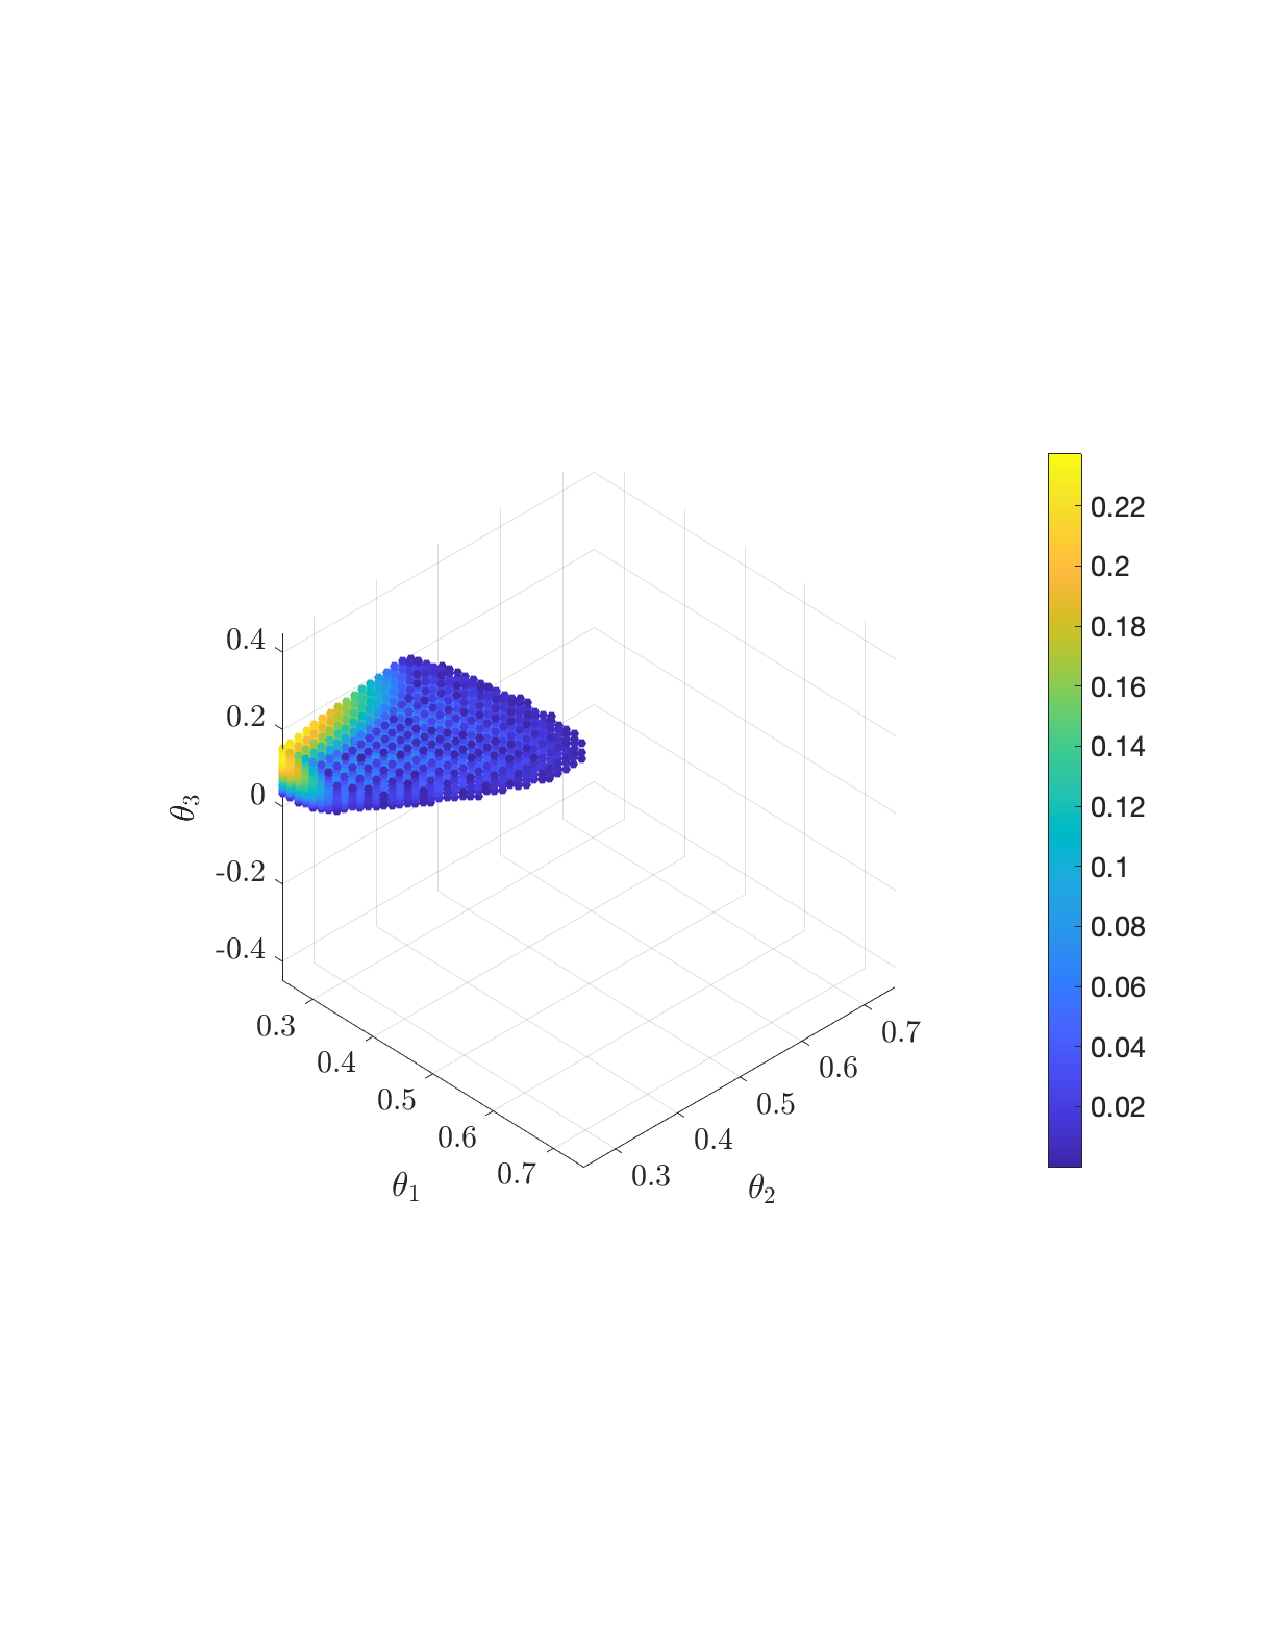
\includegraphics[width=0.8\columnwidth]{vanderpol_uncertain_theta_v3.pdf} \\
    (a) $\nu = 3$ \\

    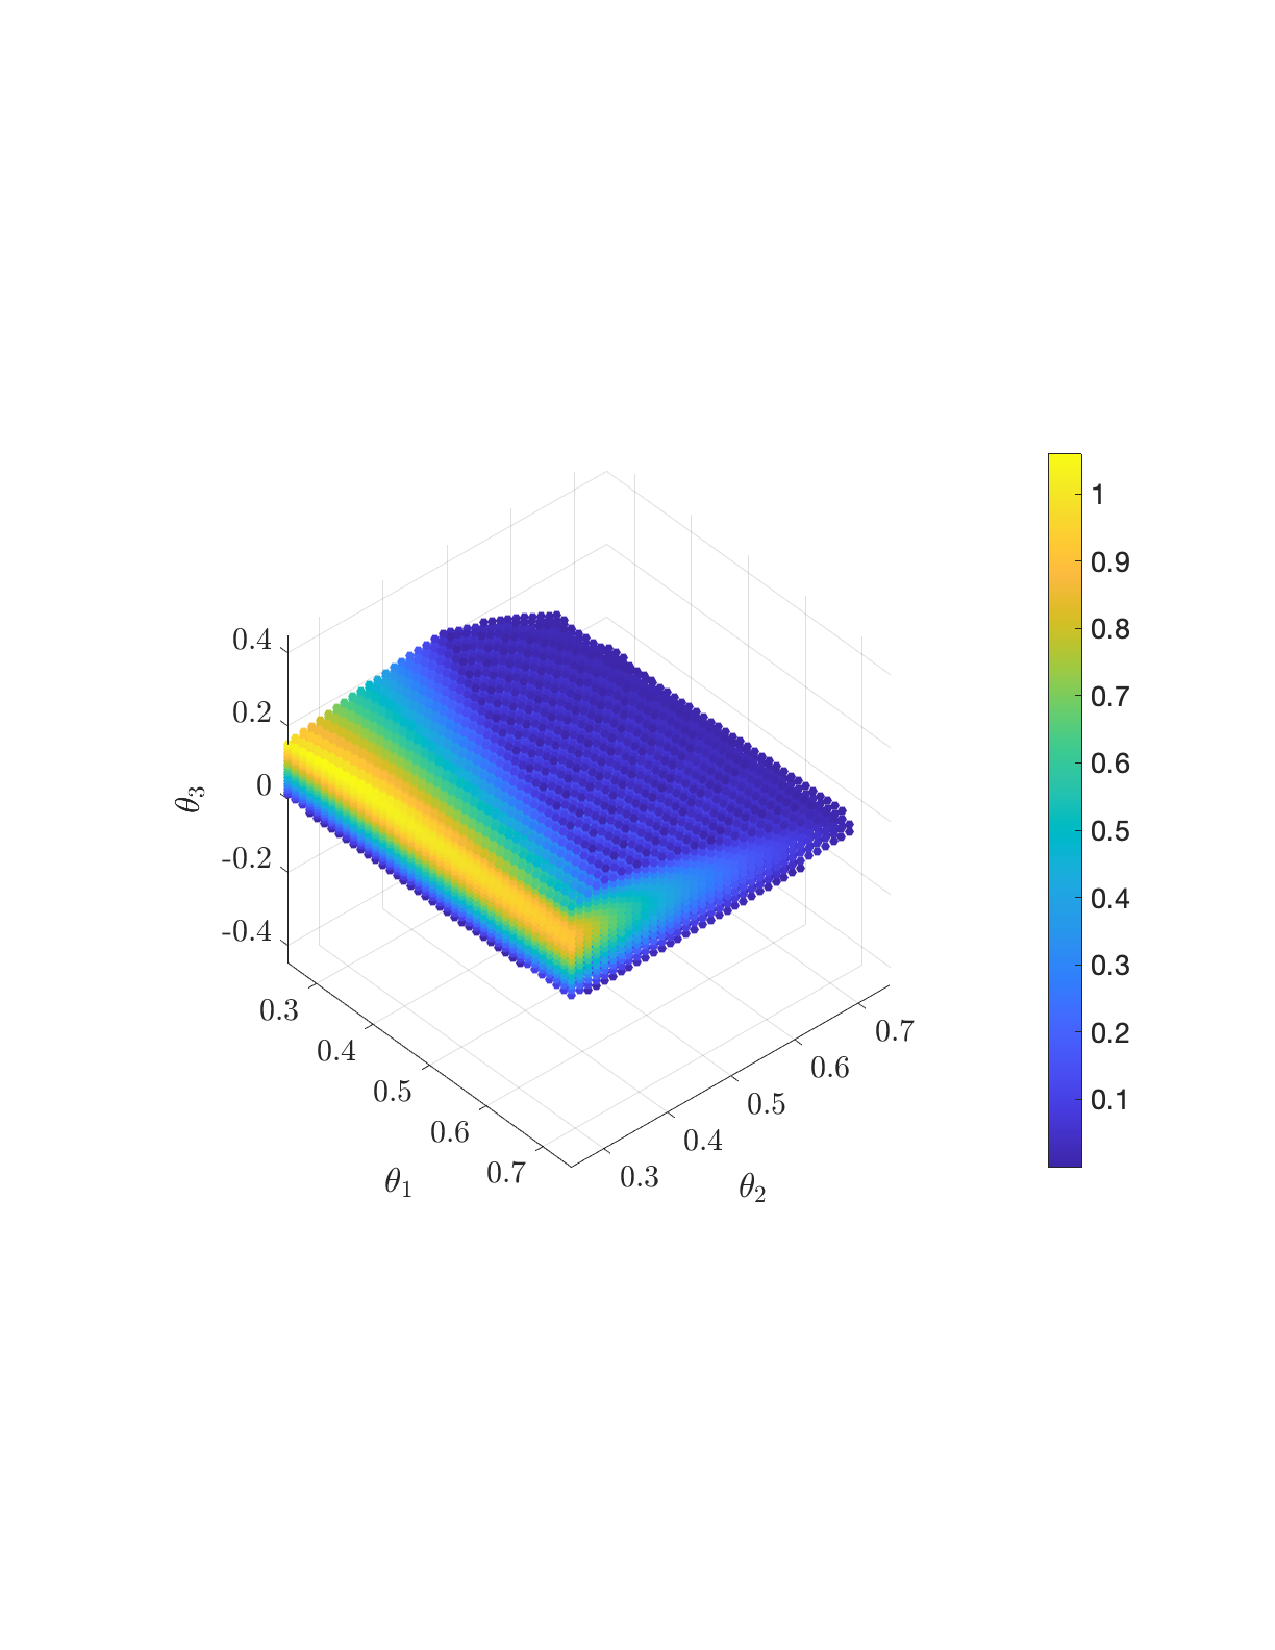
\includegraphics[width=0.8\columnwidth]{vanderpol_uncertain_theta_v4.pdf} \\
    (b) $\nu = 4$

    \caption{
        无不确定性的受控Van der Pol振荡器中~\eqref{eq:vdpodynamics},椭圆形控制障碍函数$b(x,\theta) = 1 - x^T A x$所对应的综合问题。
        \label{fig:vanderpol_uncertain}
    }
\end{figure}
